\documentclass[12pt,a4paper]{article}
\usepackage[utf8]{inputenc}
\usepackage[T2A]{fontenc}
\usepackage[russian,english]{babel}
\usepackage{amsmath}
\usepackage{amsfonts}
\usepackage{amssymb}
\usepackage{graphicx}
\usepackage[left=2cm,right=2cm,top=2cm,bottom=2cm]{geometry}
\usepackage{calc}
\usepackage{setspace}
\usepackage{indentfirst}
\usepackage{caption}
\usepackage{xcolor}
\usepackage[unicode]{hyperref}
\usepackage{minted}

\definecolor{codebg}{rgb}{0.96,0.96,0.96}  % светлый фон
\definecolor{textcolor}{rgb}{0.1,0.1,0.1}   % тёмный текст

\setminted{
    bgcolor=codebg,
    fontsize=\small,
    breaklines=true,
    frame=lines,
    framesep=2mm,
    baselinestretch=1.2,
    encoding=utf8
}

\usemintedstyle{tango}  % стиль с хорошей контрастностью


% Стиль для C++
\newminted{cpp}{
    commentstyle=\color{gray},  % серые комментарии
    keywordstyle=\color{blue!70!black},  % тёмно-синие ключевые слова
    stringstyle=\color{red!70!black},     % тёмно-красные строки
    identifierstyle=\color{textcolor},    % основной текст
    numberstyle=\color{gray!60},          % номера строк
    showspaces=false,
    showtabs=false
}

% Стиль для NASM
\newminted{nasm}{
    commentstyle=\color{gray},          % серые комментарии
    keywordstyle=\color{blue!70!black}, % тёмно-синие ключевые слова
    stringstyle=\color{red!70!black},   % тёмно-красные строки
    identifierstyle=\color{textcolor},  % основной текст
    numberstyle=\color{gray!60},        % номера строк
    showspaces=false,
    showtabs=false,
    linenos=true,
    numbersep=5pt,
    morekeywords={
        section,global,extern,equ,times,
        db,dw,dd,dq,resb,resw,resd,resq,
        mov,push,pop,call,ret,jmp,jz,jnz,je,jne,
        add,sub,mul,div,inc,dec,
        eax,ebx,ecx,edx,esi,edi,esp,ebp,
        rax,rbx,rcx,rdx,rsi,rdi,rsp,rbp
    }
}

% Стиль для Bash
\newminted{bash}{
    commentstyle=\color{gray},          % серые комментарии
    keywordstyle=\color{blue!70!black}, % тёмно-синие ключевые слова
    stringstyle=\color{red!70!black},   % тёмно-красные строки
    identifierstyle=\color{textcolor},  % основной текст
    numberstyle=\color{gray!60},        % номера строк
    showspaces=false,
    showtabs=false,
    linenos=true,
    numbersep=5pt,
    morekeywords={
        if,then,else,fi,for,while,do,done,
        case,esac,function,select,until,
        echo,export,read,printf,test,
        cd,ls,mkdir,rm,cp,mv,chmod,chown,
        grep,awk,sed,find,ssh,scp
    }
}

\title{
    Отчет о выполнении лабораторной работы 3565.32.50494452
    
    Оценка эффективности SIMD-оптимизаций программы Mandelbrat2
    }
    
\author{Швабра Владимир Сергеевич, Б01-411}

\captionsetup[figure]{name=Рис.}

\begin{document}
\maketitle

\newpage

\tableofcontents

\newpage

\section{Аннотация}
\subsection{Цели работы}  
\begin{enumerate}
    \item Научиться применять различные низкоуровневые оптимизации на примере расчёта множества Мандельброта.
    \item Научиться оценивать эффективность работы программы
\end{enumerate}

\subsection{Теоретическая справка}

Сначала рассмотрим базовую последовательную 5-ступенчатую модель выполнения инструкций (SEQ, Sequential Execution Model), а затем перейдем к современным конвейерным реализациям (PIPE, Pipelined Execution) с предсказанием переходов. Далее будет описано 6 этапов а не 5. Это решение было принято, чтобы акцентировать внимание на выборе нового PC (Program Counter, счётчик команд).

\subsubsection{Последовательная модель выполнения (SEQ)}
На рисунке \ref{fig:seq} представлена последовательная модель обработки инструкций:

\begin{figure}[ht!]
\centering
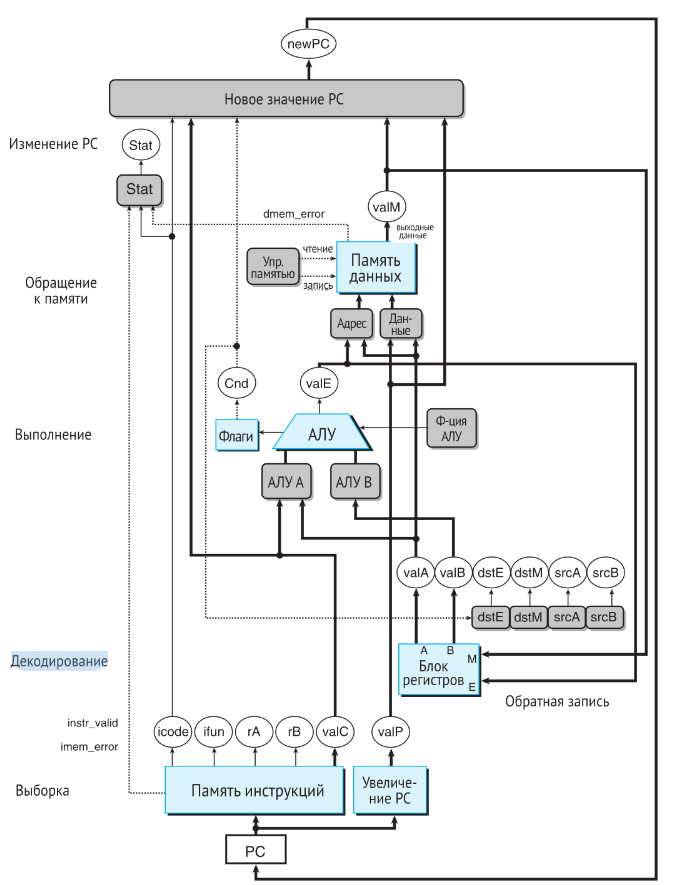
\includegraphics[width=0.9\textwidth]{seq.png}
\caption{Блок-схема последовательной обработки инструкций (SEQ)[2]}
\label{fig:seq}
\end{figure}

\paragraph{Этапы последовательной обработки}

\begin{enumerate}
    \item \textbf{Выгрузка (F, Fetch)}:
    \begin{itemize}
        \item Извлекает инструкцию из памяти по адресу, указанному в Program Counter (PC)
        \item Используется \textit{кэш инструкций} для ускорения доступа
        \item PC увеличивается на размер инструкции (или изменяется для инструкций перехода)
    \end{itemize}

    \item \textbf{Декодирование (D, Decode)}:
    \begin{itemize}
        \item Определяется \textit{тип операции} (арифметическая, логическая, перехода и т.д.)
        \item Выявляются \textit{операнды} (регистры, непосредственные значения, адреса памяти)
        \item Для операций с памятью вычисляются эффективные адреса
        \item Подготавливаются сигналы управления для следующих этапов
    \end{itemize}

    \item \textbf{Выполнение (E, Execute)}:
    \begin{itemize}
        \item Выполнение арифметических или логических операций в \textit{АЛУ} (Арифметико-Логическом Устройстве, ALU - Arithmetic Logic Unit)
        \item Для условных переходов - проверка условий и вычисление адреса перехода
    \end{itemize}

    \item \textbf{Обращение к памяти (M, Memory)}:
    
    Этот этап присутствует только для инструкций работы с памятью.
    \begin{itemize}
    \item Для загрузки: чтение данных из памяти по вычисленному адресу
    \item Для записи: запись данных в память по вычисленному адресу
    \item Используется \textit{кэш данных} для ускорения доступа
    \item Обработка кэш-промахов и обращение к основной памяти при необходимости
    \end{itemize}

    \item  \textbf{Обратная запись (W, Writeback)}:
    \begin{itemize}
        \item Для арифметических операций - запись в регистр-приемник
        \item Для операций загрузки - запись данных из памяти в регистр
    \end{itemize}

    \item \textbf{Изменение PC}:
    \begin{itemize}
        \item Для обычных инструкций: PC уже был увеличен на этапе выгрузки
        \item Для инструкций перехода: PC изменяется на новое значение
        \item Для условных переходов: PC изменяется только если условие истинно
        \item Обработка исключений и прерываний также может изменить PC
    \end{itemize}
\end{enumerate}

\paragraph{Ограничения SEQ.}
Главный недостаток последовательной модели — низкая эффективность. Каждый этап задействует только часть аппаратных ресурсов процессора, остальные простаивают.

\subsubsection{Конвейерная модель выполнения (PIPE)}
Современные процессоры используют конвейерную обработку, как показано на рисунке \ref{fig:pipe}.

\begin{figure}[ht!]
\centering
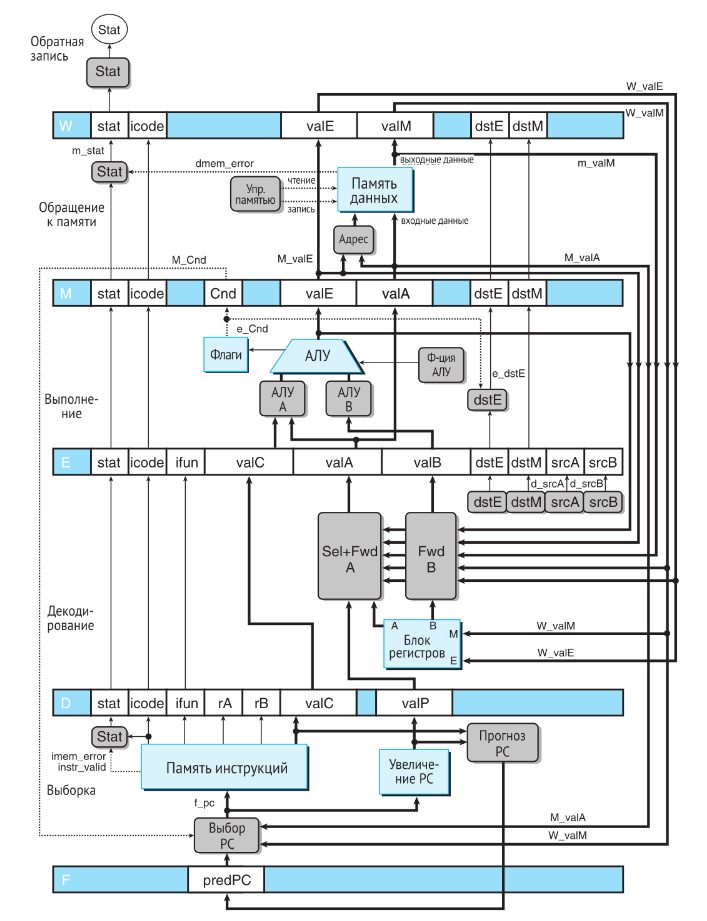
\includegraphics[width=0.8\textwidth]{pipe.png}
\caption{Блок-схема конвейерной обработки инструкций (PIPE)[2]}
\label{fig:pipe}
\end{figure}

Из общих изменений в схеме добавились конвейерные регистры между каждой соседней парой этапов обработки инструкций. Это сделано для возможности выполнения разных этапов разных инструкций параллельно, как показно на рисунке \ref{fig:pipeline}.

\begin{figure}[ht!]
    \centering
    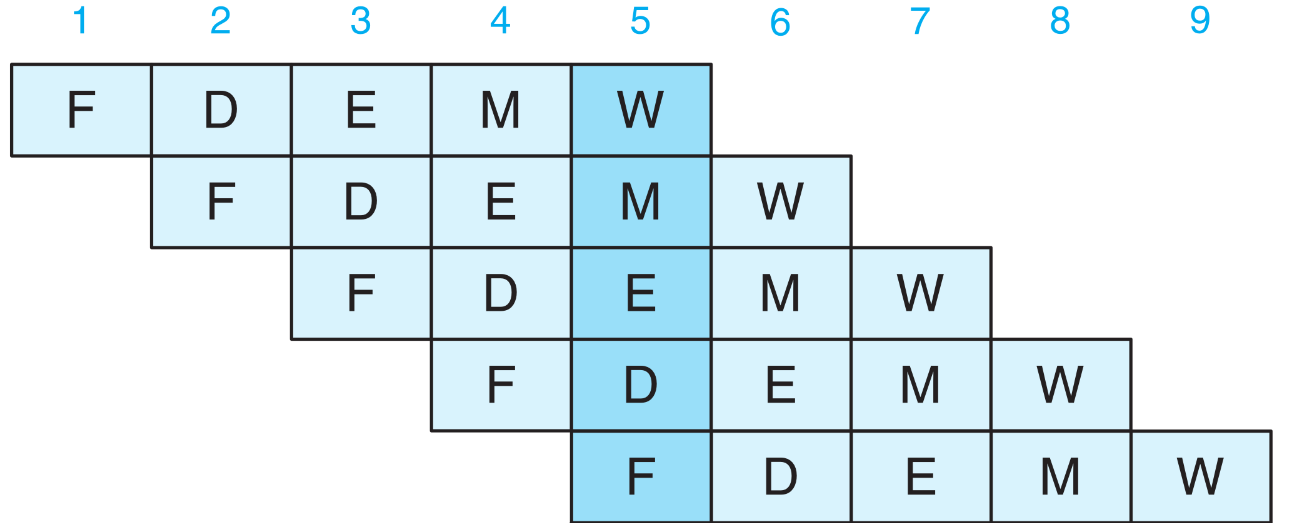
\includegraphics[width=0.8\textwidth]{pipeline.png}
    \caption{Визуализация конвейерной обработки инструкций[2]}
    \label{fig:pipeline}
\end{figure}

\paragraph{Предсказание РС.}
\indent

Если обрабатываемая инструкция не является условным переходом, то мы можем однозначно определить следующее значение PC, но иначе нет.

\begin{itemize}
    \item \textbf{Инструкции не выполняющие "прыжок" - } так как мы знаем размер каждой инструкции, то можем прибавить его к PC.
    \item \textbf{CALL, JMP - } мы знаем адрес, на который нужно перейти в случаях, когда операндами являются литералы. Иначе мы не знаем куда прыгать.
    \item \textbf{Условный переход - } До проверки условия мы не знаем куда надо делать "прыжок".
    \item \textbf{RET - } также не знаем куда куда нужно возвращаться, так как адрес возврата в стеке можно менять.
\end{itemize}

Проблему с условными переходами можно решить приостановкой загрузки новых инструкций в конвейер до момента вычисления условия, но есть решение лучше. Мы попробуем угадать произойдёт переход или нет и продолжать подгружать операции с соответствующего места, а в случае ошибочного предсказания сбросить загруженные инструкции, что, конечно, ударит по производительности.

Существует много различных стратегий для предсказания переходов (branch prediction), но мы не будем в это углубляться. Отметим лишь, что для облегчения работы предсказателю, не стоит писать сложных условий без необходимости. Также нужно знать об операциях условного перемещения (conditional move), которые могут улучшить производительность ветвлений.

\paragraph{Риски по данным (data hazards).}
\indent 

Но схема на рисунке \ref{fig:pipeline} будет работать корректно только если во всех инструкциях, которые выполняются параллельно не будет \textit{зависимости по данным}, что может часто не соблюдаться. Приведём методы разрешения таких зависимостей.

\begin{itemize}
    \item \textbf{NOP (No Operation):} самое лёгкое решение. На этапе генерации ассемблера проставить пустые инструкции в количестве необходимом, для такого чтобы устранить параллельное выполнение инструкций зависимых по данным (Рис. \ref{fig:nop}).
    \begin{figure}[ht!]
        \centering
        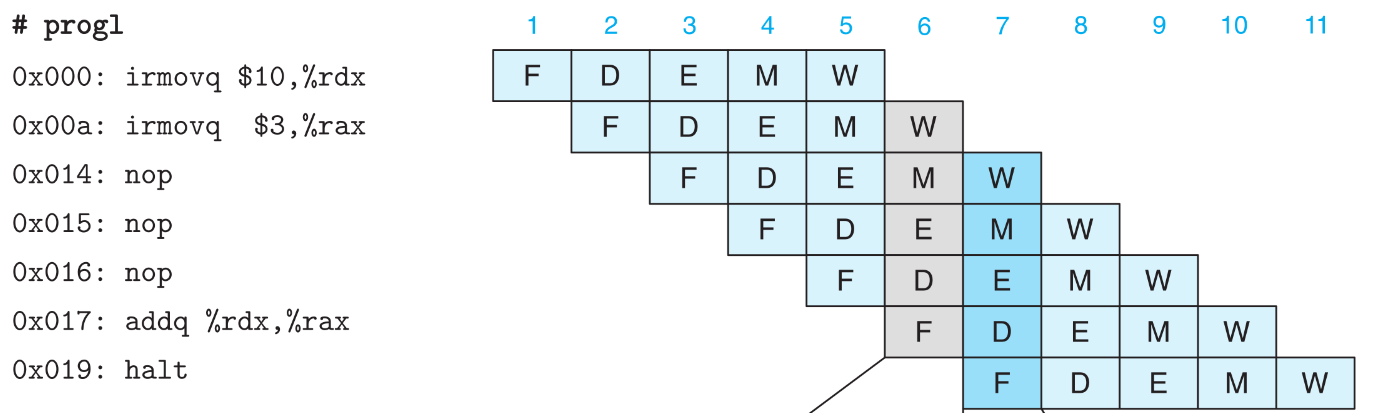
\includegraphics[width=0.8\textwidth]{nop.png}
        \caption{Останова, реализованная через NOP для решения проблемы риска по данным[2]}
        \label{fig:nop}
    \end{figure}

    \item \textbf{"Пузырёк" (bubble, Привет дед!): } Аппаратная приостановка конкретных этапов обработки инструкций, зависящих по данным (Рис. \ref{fig:babble}).
    \begin{figure}[ht!]
        \centering
        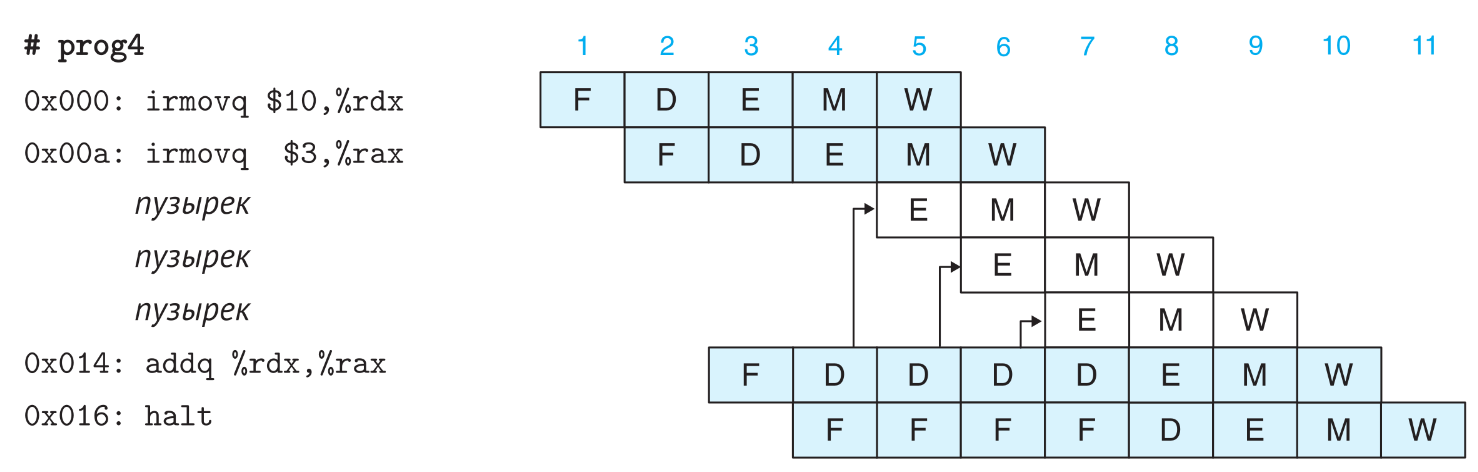
\includegraphics[width=0.8\textwidth]{babble.png}
        \caption{Останова, реализованная через "пузырёк" для решения проблемы риска по данным[2]}
        \label{fig:babble}
    \end{figure}

    \item \textbf{Продвижение (forwarding): } Мы добавляем в нашу конструкцию процессора (Рис. \ref{fig:pipe}) возможность передачи значений (регистров, либо памяти) в предыдущие этапы обработки инструкций, чтобы ожидающая инструкция могла использовать уже вычисленное значение до окончания обработки ожидаемой инструкции (Рис. \ref{fig:forwarding}).
    \begin{figure}[ht!]
        \centering
        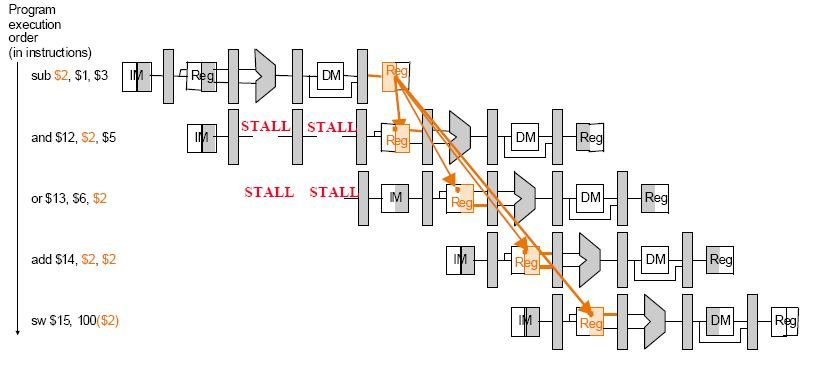
\includegraphics[width=0.8\textwidth]{forwarding.png}
        \caption{Визуализация продвижения назад при зависимости по данным[3]}
        \label{fig:forwarding}
    \end{figure}
\end{itemize}

\paragraph{Взаимосвязь функциональных блоков.}
\indent

В настоящих процессорах, очевидно, есть несколько функциональных блоков, каждый из которых занимается обработкой операций того или иного типа. Это позволяет выполнять некоторые операции не по порядку. Такая архитектура процессора называется суперскалярной (superscalar, Рис \ref{fig:superscalar}) и хорошо дополняет конвейерное устройство функциональных блоков.

Распределением инструкций по функциональным блокам занимается \textit{блок управления инструкциями (БУИ (это я ввёл сам, так не называют, просто чтобы меньше писать (лисп сосать (дед упрлс (а стоп, это же не гайд на летку (ну ладно, пока (швабра))))))} (Instruction Control Unit). В частности на всех современных процессорах есть блок для обработки ветвлений, который пытается предсказать условные переходы (аналогично предсказателю PC в рамках одного конвейера, но на уровень выше). Такая организация обработки инструкций называется \textit{спекулятивным выполнением (speculative execution)}.

\begin{figure}[ht!]
    \centering
    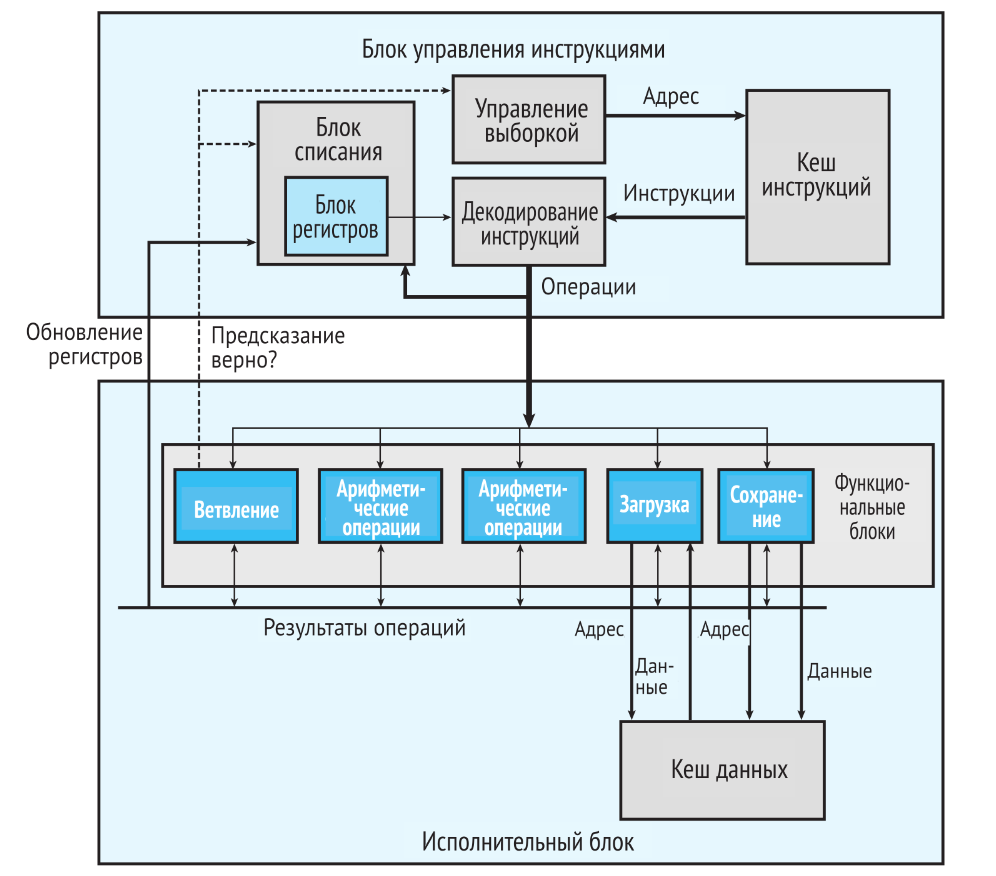
\includegraphics[width=0.8\textwidth]{supscalar.png}
    \caption{Блок-схема суперскалярного процессора[2]}
    \label{fig:superscalar}
\end{figure}


\subsubsection{Оптимизации}

На основе знаний изложенных выше мы можем "класть" наш код на аппаратуру применением низкоуровневых оптимизаций, чтобы увеличить производительность. Некоторые из них мы сейчас опишем


\paragraph{Вынос кода (code motion).}

Если в цикле вычисляется значение переменной и не меняется на всех итерациях цикла, то для данного значения стоит завести константу вне цикла и использовать её. Аналогично можно поступить при постоянном обращении к памяти, правда это будет эффективно в случае, если есть свободные регистры для сохранения переменной.

\newpage

\begin{minted}{cpp}
// До оптимизации
for (size_t i = 0; i < n; ++i) {
    double result = sin(x) * arr[y] + i;  // sin(x) и arr[y] не зависят от i
    printf("%f\n", result);
}

// После оптимизации
double sin_x = sin(x);
double arr_y = arr[y];
for (size_t i = 0; i < n; ++i) {
    double result = sin_x * arr_y + i;
    printf("%f\n", result);
}
\end{minted}

\paragraph{Уменьшение рисков по данным (data hazards reduction).}

Стоит уметь представлять в голове как конвейерная и суперскалярная архитектура будут обрабатывать инструкции и минимизировать простои процессора. Допустим, если есть возможность переставить вычисление независимых операций, то их можно поставить между зависимыми, чтобы занять неиспользуемое время.

\begin{minted}{cpp}
// До оптимизации
float x = y * z;  // Независимая операция
float a = b * c;
float d = a + e;  // Зависит от a

// После оптимизации
float a = b * c;
float x = y * z;   // Независимая операция
float d = a + e;
\end{minted}

\paragraph{Комбинация развёртывания цикла (loop unrolling) и аккумулятора (accumulator).}
\indent

\textbf{Развёртывание: } это преобразование программы, которое уменьшает количество итераций за счет увеличения количества вычислений в каж­дой итерации. Развертывание цикла может улучшить производительность по двум причинам. Во-первых, уменьшается количество операций, не влияющих непосредственно на результат программы, таких как вычисление индекса и условное ветвление. Во-вторых, открываются возможности для дальнейшего преобразования кода при помощи аккумуляторов.

\textbf{Аккумуляторы: } Для ассоциативной и коммутативной комбинирующей операции (например для целочисленного сложения или умножения) производительность можно повысить, разбив набор комбинирующих операций на две или более частей, и комбинировать их результаты в конце. 

Без учёта накладных расходов использование описанных подходов можно увеличить скорость выполнения цикла во столько раз, на сколько порядков проведено развёртывание. Конечно, это можно делать не бесконечно, ведь в какой-то момент регистров для аккумуляторов не будет хватать и они будут сохраняться в переменные, что только замедлит обработку инструкций. Подробную оценку производительности читайте в БХ (байт для будущих пекусов).

\begin{minted}{cpp}
// До оптимизации
float sum = 0;
for (int i = 0; i < n; i++) {
    sum += array[i];
}

// После оптимизации (развёртывание 4x + аккумуляторы)
float sum0 = 0, sum1 = 0, sum2 = 0, sum3 = 0;
for (int i = 0; i < n; i += 4) {
    sum0 += array[i];
    sum1 += array[i+1];
    sum2 += array[i+2];
    sum3 += array[i+3];
}
float sum = sum0 + sum1 + sum2 + sum3;
\end{minted}

\paragraph{Применение векторных инструкций (SIMD, Single Instruction Multiple Data).}

Модель выполнения инструкций SIMD позволяет производить одну операцию сразу с несколькими данными в соответствующих функциональных блоках с поддержкой векторных операций. Использование таких инструкций очень хорошо сочетается с вышеперечисленными оптимизациями.

\begin{minted}{cpp}
#include <immintrin.h>

// До оптимизации
for (int i = 0; i < n; i++) {
    c[i] = a[i] + b[i];
}

// После оптимизации
for (int i = 0; i < n; i += 4) {
    __m128 va = _mm_load_ps(&a[i]);
    __m128 vb = _mm_load_ps(&b[i]);
    __m128 vc = _mm_add_ps(va, vb);
    _mm_store_ps(&c[i], vc);
}
\end{minted}

\subsubsection{Измерение эффективности.}

Наиболее точным способом измерения времени работы программы является ассемблерная инструкция \textit{rdtsc (Read Time-Stamp Counter)}, которая возвращает количество пройденных тактов с момента запуска программы. Проблема состоит в том, что тактовая частота при нормальной работе машины постоянно меняется. Мы можем зафиксировать её специальными утилитами (далее для ОС Fedora).

\begin{minted}{bash}
    # Установка нужных инструментов
    $ sudo dnf install kernel-tools cpupowerutils

    # Вывод информации о процессоре
    $ cpupower frequency-info
    analyzing CPU 0:
    #...
    hardware limits: 400 MHz - 3.60 GHz
    #...
    current CPU frequency: 2.23 GHz (asserted by call to kernel)
    #...
    # Несколько раз потыкав внешнюю программу можно понять какую максимальную частоту можно поставить, чтобы она не менялась. Я выбрал 1 GHz

    $ sudo cpupower frequency-set -u 1.0GHz

    # Проверям
    $ cpupower frequency-info

\end{minted}

После работы возвращаем всё на свои места, ставя ограничение на максимальную частоту больше, чем может быть максимум

\begin{minted}{bash}
    $ sudo cpupower frequency-set -u 3.6GHz
\end{minted}

Стоит уточнить, что измерение будет производиться на одном и том же "месте" множества мандельброта и при одинаковых параметрах экрана, чтобы расчёты были идентичными.

\section{Оборудование}

\begin{itemize}
    \item \href{https://adrenalinerush.ru/}{2 банки энергетика}
    \item \href{http://ded32.net.ru/}{конспекты деда}
    \item \href{https://www.tver.ru/info/prokuratura/proletarskiy-rayon/razyasneniya/39923/}{18+ бутылка пива}
    \item \href{https://github.com/71frukt}{чипсы соседа}
    \item третье издание БХ [2]
    \item \href{https://www.mirpruzhin.ru/}{слинки (всем с СДВГ советую)}
    \item ноутбук (опционально) (Рис. \ref{fig:nout})
    \begin{figure}[ht!]
        \centering
        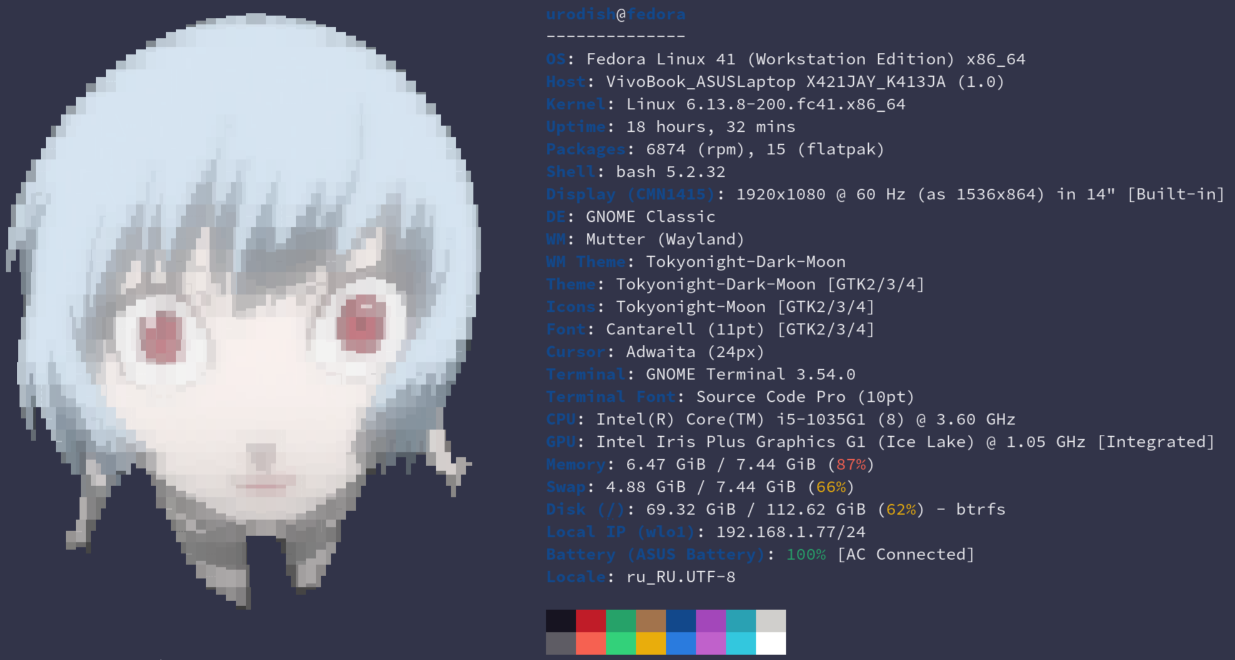
\includegraphics[width=0.8\textwidth]{nout.png}
        \caption{Характеристики ноутбука, на котором выполняется работа}
        \label{fig:nout}
    \end{figure}
\end{itemize}

\section{Ход работы}

\subsection{Зависимости}

Для сборки проекта нужны Make и GCC (GNU Compiler Collection). Для отрисовки множества Мандельброта возьмём библиотеку SDL2 (Simple DirectMedia Layer 2) (SFML для лохов), также дополнительно установим модуль TTF (TrueType Font) для вывода FPS (Frames Per Second) на экран.

\subsection{Начало работы. Поверхностная оценка производительности}

Основным местом, которое мы будем оптимизировать является функция расчёта самого множества. Накладные расходы по типу инициализации SDL и логгера, обработки флагов и отрисовки множества мы не будем учитывать при измерении эффективности, так как это не цель исследования. Соответственно, максимально постараемся минимизировать их вклад в измеряемую производительность.


\subsubsection{Нулевая версия} 

Напишем наивную версию программы и настроим на её основе:
\begin{itemize}
    \item Обработку флагов, чтобы можно было изменять параметры отображения множества Мандельброта, отключать графику и увеличивать количество повторных обработок 1 кадра (для увеличения точности измерений)
    \item Движение по множеству, а также приближение или отдаление к центру координат, чтобы было удобнее рассматривать математические красоты
    \item Вывод текущего FPS, чтобы примерно оценить скорость расчёта кадров без точных времязатраных измерений, реализованный через функции SDL2.
\end{itemize}

\begin{figure}[ht!]
    \centering
    
\includegraphics[width=0.5\textwidth]{mand_O0.png}
    \caption{Визуализация множества Мандельброта без оптимизаций}
    \label{fig:mand_O0}
\end{figure}

В среднем значение FPS варьируется в районе 3.5 FPS на изначальной позиции, то есть без сдвига системы координаты и без приближения. В дальнейшем мы будем использовать эту позицию для всех измерений, чтобы они проводились в одинаковых условиях.

\subsubsection{Наивные оптимизации} 

Теперь мы можем начать оптимизировать программу. Для начала применим оптимизации, которые не требуют переписывания кода. А именно установим уровень оптимизации -O3, пропишем флаги, которые позволят компилятору применять дополнительные оптимизации, а также сделаем предварительный запуск программы, чтобы применить оптимизацию профилировщиком (Profile-guided optimization, PGO), далее будем называть PGO.

При первом запуске профилировщик будет "анализировать" как выполняется программа и предполагать какие решения могут её ускорить. К примеру это может сильно ускорить ветвления, так как будет заранее известно когда выполняется условие. Эта информация записывается в файл, который используется при втором запуске.

\begin{figure}[ht!]
    \centering
    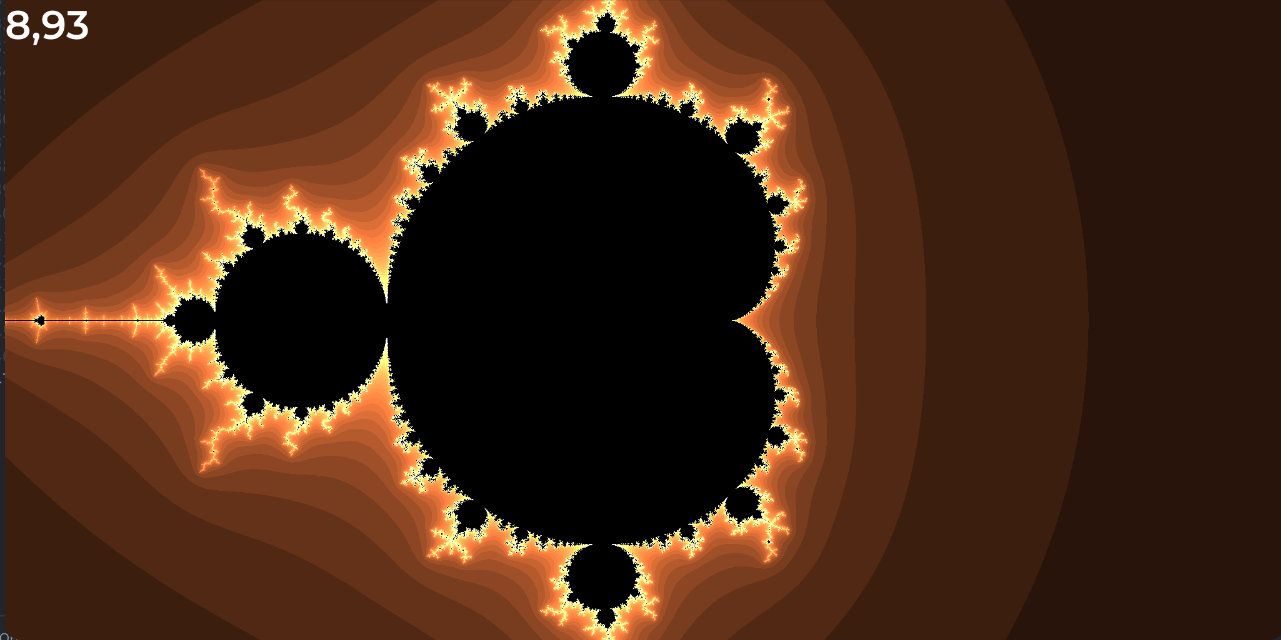
\includegraphics[width=0.5\textwidth]{mand_O3.png}
    \caption{Визуализация множества Мандельброта c наивными оптимизациями}
    \label{fig:mand_O3}
\end{figure}

Значение FPS находится в районе 7.5-8.

\subsubsection{Векторные инструкции (AVX2)} 

Теперь начнём применять оптимизации, для которых придётся изменять код, и, к сожалению, приводить его к менее читаемому виду. Задействуем функциональный блок, который умеет обрабатывать SIMD-инструкции и перепишем код на интринсиках (intrinsics). Это специальные функции, которые вместо себя подставляют соответствующую ассемблерную инструкцию. Эти инструкции являются аппаратно-зависимыми, поэтому для различных процессоров будет свой список и свои названия. Характеристики машины, которая используется в данной работе, приведены в главе Оборудование.

Будем использовать тип \verb|__m256|, который сможет хранить 8 значений типа \verb|float|. Соответственно итоговый прирост к скорости должен быть примерно в 8 раз по сравнению с прошлой версией без учёта накладных расходов.

\begin{figure}[ht!]
    \centering
    
\includegraphics[width=0.5\textwidth]{mand_avx2.png}
    \caption{Визуализация множества Мандельброта на интринсиках}
    \label{fig:mand_avx2}
\end{figure}

FPS вырос примерно в 4 раза, а не в 8. Это можно объяснить тем, что отрисовка пикселей и обработка событий SDL2 сравнима по времени выполнения с исследуемыми расчётами. Следовательно, далее анализировать показатель FPS не имеет смысла, так как он некорректно показывает вклад применённых оптимизаций.

\subsubsection{Развёртывание (loop unrolling)} 

Мы уже применили векторные инструкции, которые выполняются на отдельном функциональном блоке, но ведь в нашем коде невозможно полностью избежать зависимости по данным просто перестановкой операций. Поэтому, для того чтобы полностью загрузить конвейер, применим развёртывание цикла. 

\begin{figure}[ht!]
    \centering
    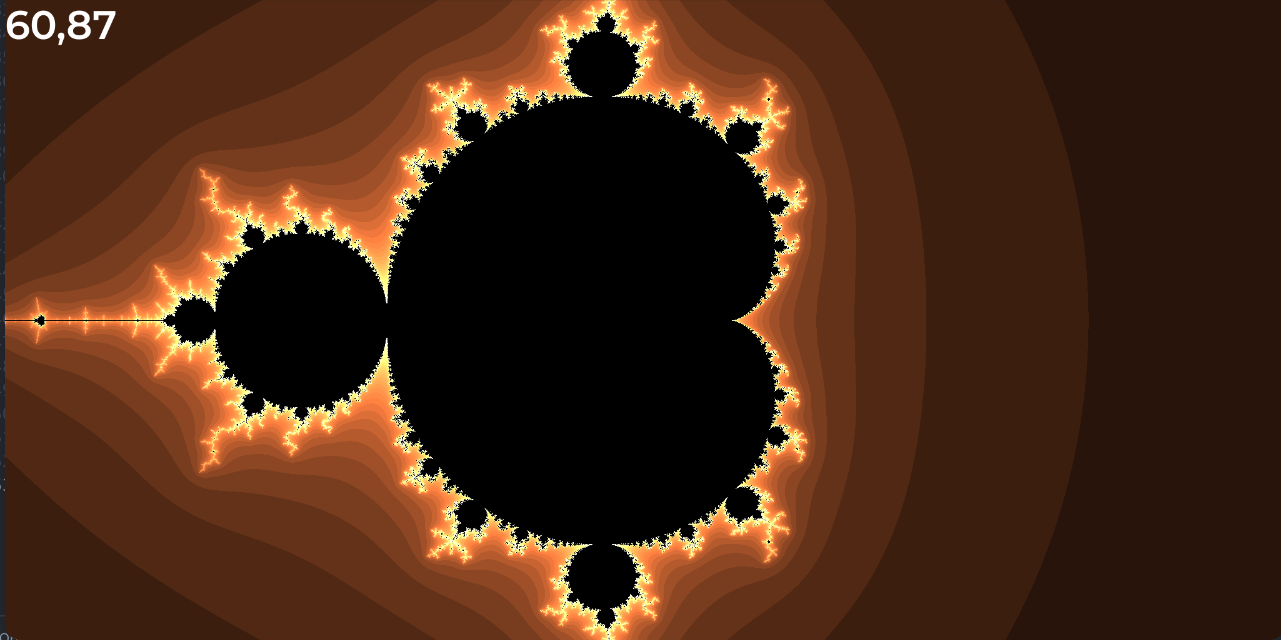
\includegraphics[width=0.5\textwidth]{mand_avx2_unroll.png}
    \caption{Визуализация множества Мандельброта на интринсиках c развёртыванием}
    \label{fig:mand_avx2_unroll}
\end{figure}

\subsubsection{Кроссплатформенность} 

Как упоминалось ранее интринсики аппаратно-зависимы. Но компилятор может сам заменять циклы на векторные операции, если заметит возможность такой оптимизации. Тогда можно написать программу на массивах размером 8, которые с первого взгляда будут только ухудшать производительность, но при правильной организации кода будут заменяться соответствующими векторными инструкциями. В таком случае код будет переносимым и не должен сильно потерять в производительности.

\begin{figure}[ht!]
    \centering
    
\includegraphics[width=0.5\textwidth]{mand_arr.png}
    \caption{Визуализация множества Мандельброта на массивах c развёртыванием}
    \label{fig:mand_arr2}
\end{figure}

FPS упал даже ниже, чем на версии с интринсиками без развёртывания (значение FPS версии программы на массивах без развёртывания было таким же). Скорее всего это произошло из-за того, что компилятор не смог заменить некоторые неочевидные аналоги векторных инструкций. Это наталкивает на идею оценить производительность при сборке разными компиляторами.

\subsection{Точная оценка производительности}

\subsubsection{Проверка стационарности}

Прежде чем проводить измерения нужно убедиться, что соблюдается стационарность процесса. Установим условия, при которых собираемся прогонять программу (частота процессора - 1Ghz, наивысший приоритет программы (nice -n -20), отключение графического режима) и построим график зависимости времени выполнения от итерации.

\begin{figure}[ht!]
    \centering
    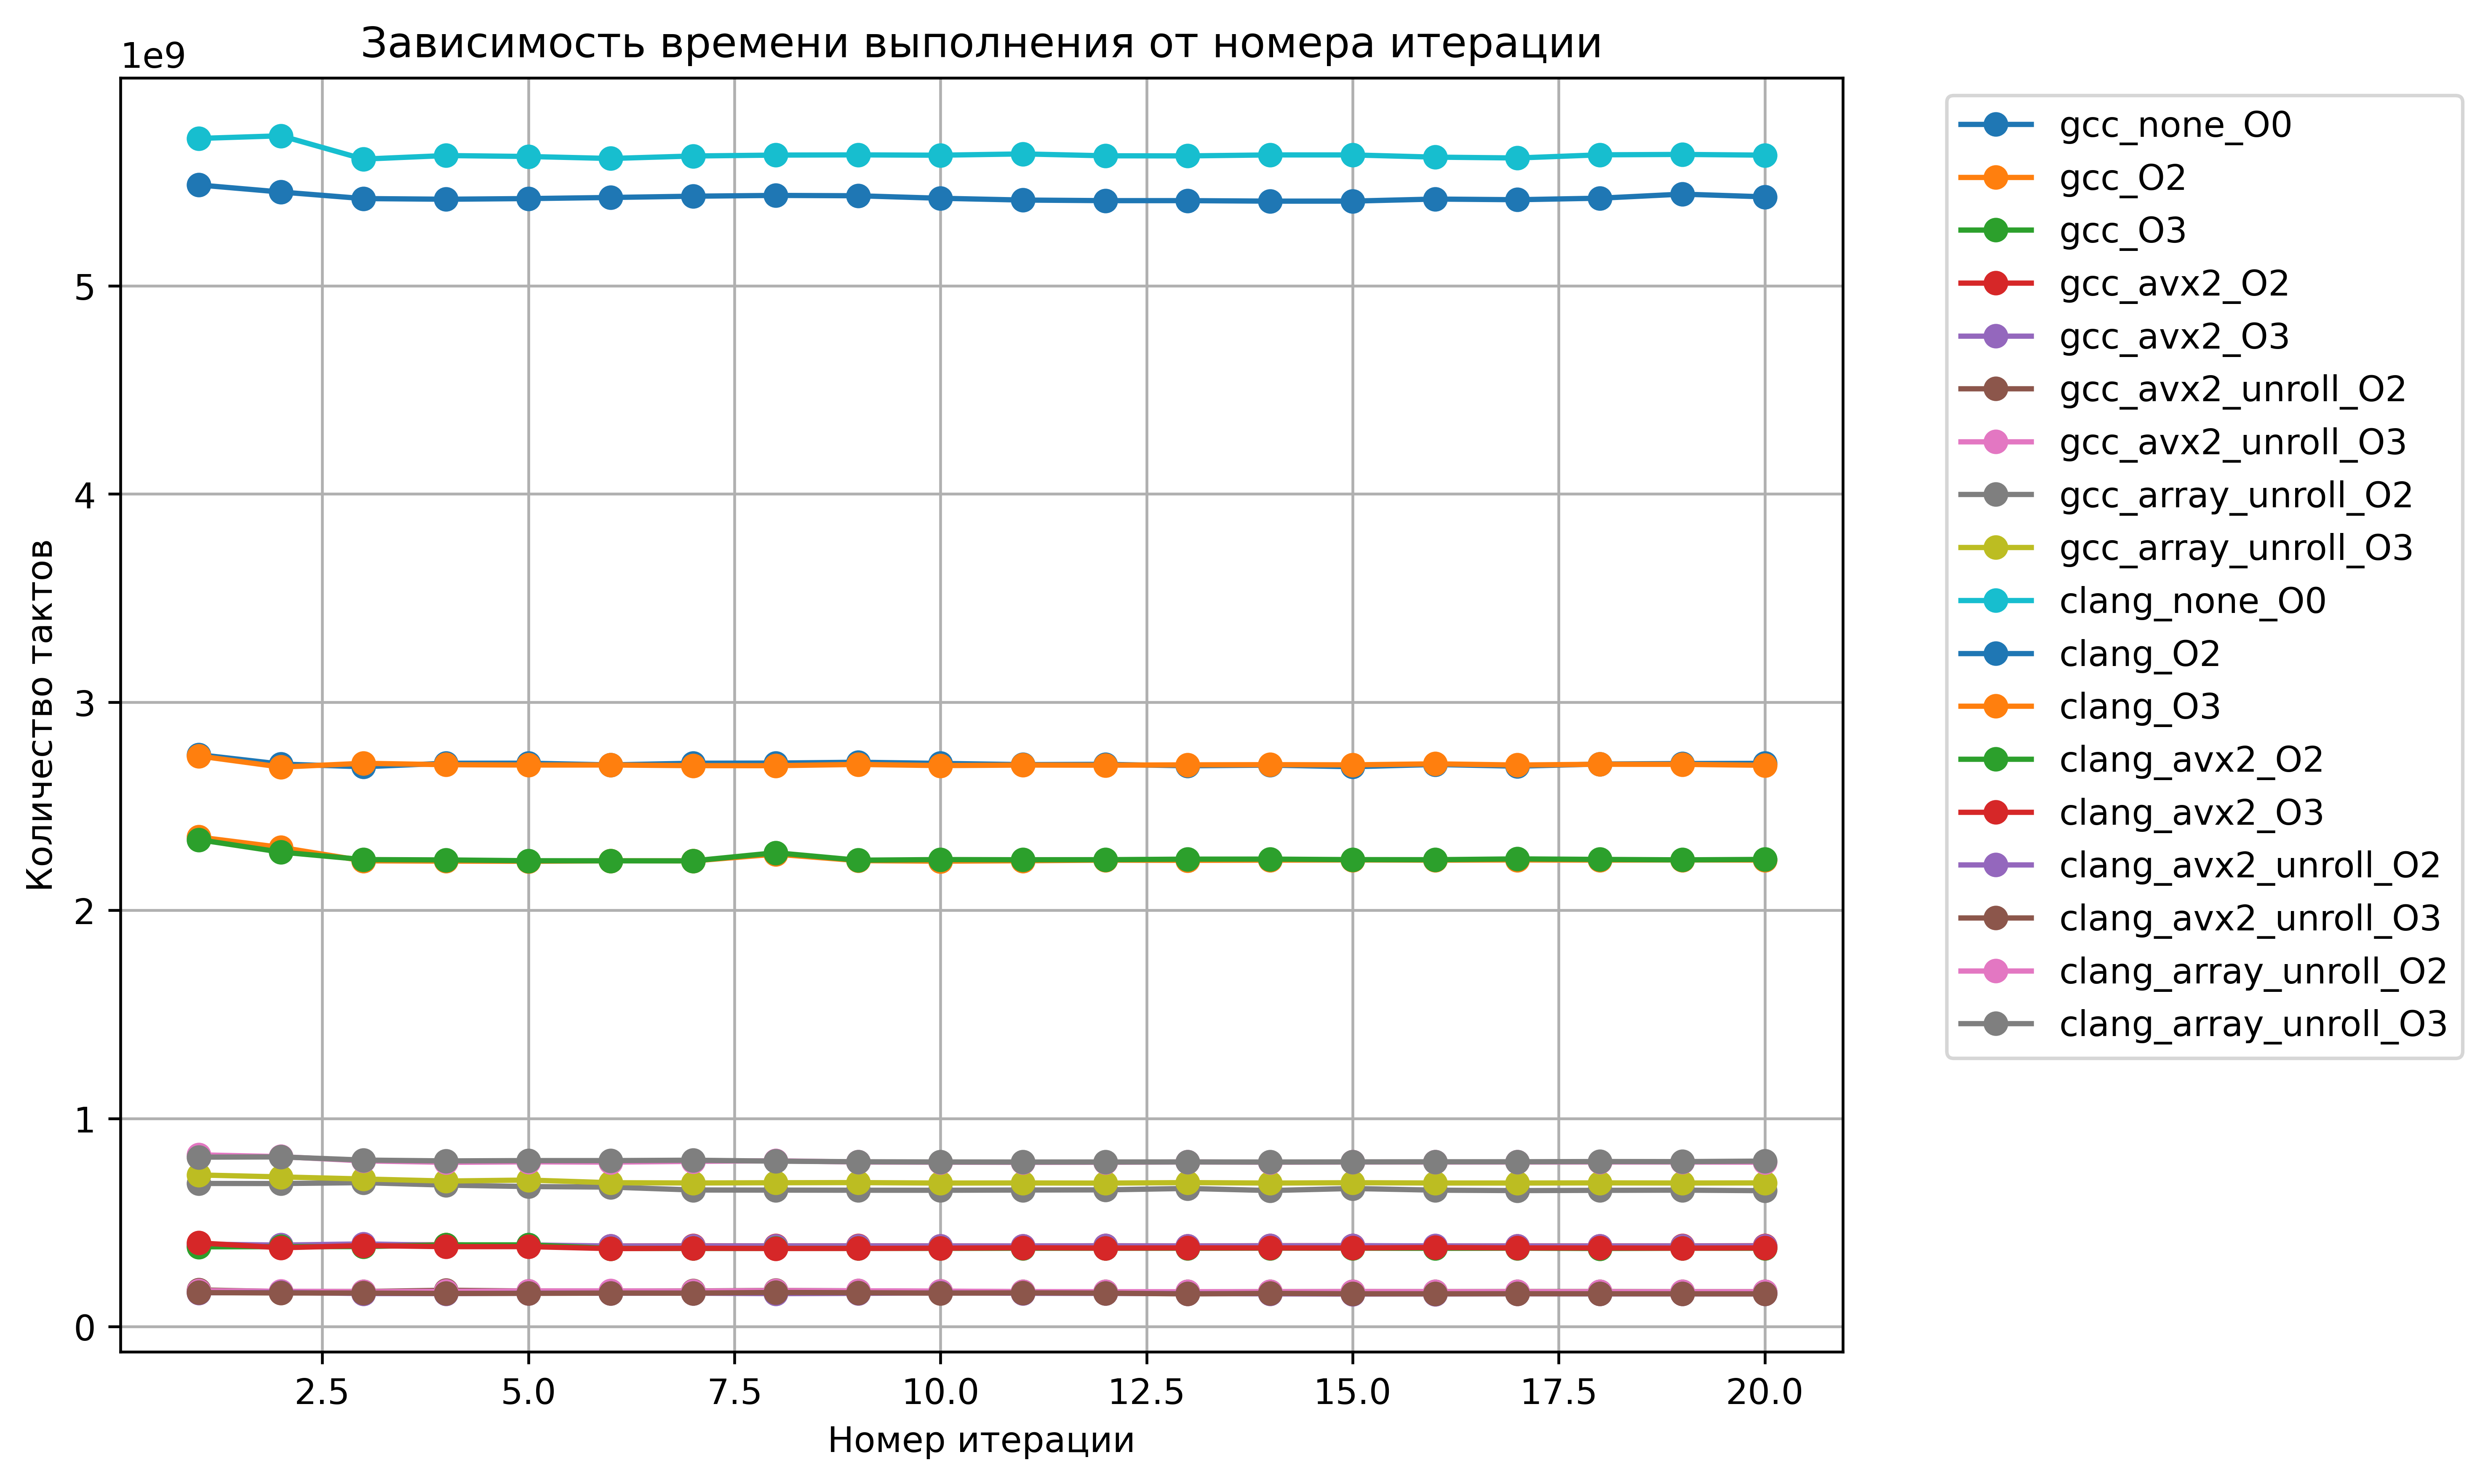
\includegraphics[width=0.8\textwidth]{stat_check.png}
    \caption{График зависимости времени выполнения от итерации}
    \label{fig:stat_check}
\end{figure}

Отклонения от нормы находится в пределах 1\%, а значит измерениям можно будет доверять.

\subsubsection{Измерения}

\paragraph{Baseline.} Имеет смысл оценивать прирост производительности оптимизаций, которые требуют переработки кода, так как оптимизирующие флаги компиляции и так используются в release-версии программы, поэтому выберем baseline, то есть версию, относительно которое будем смотреть прирост оптимизаций.

\begin{figure}[ht!]
    \centering
    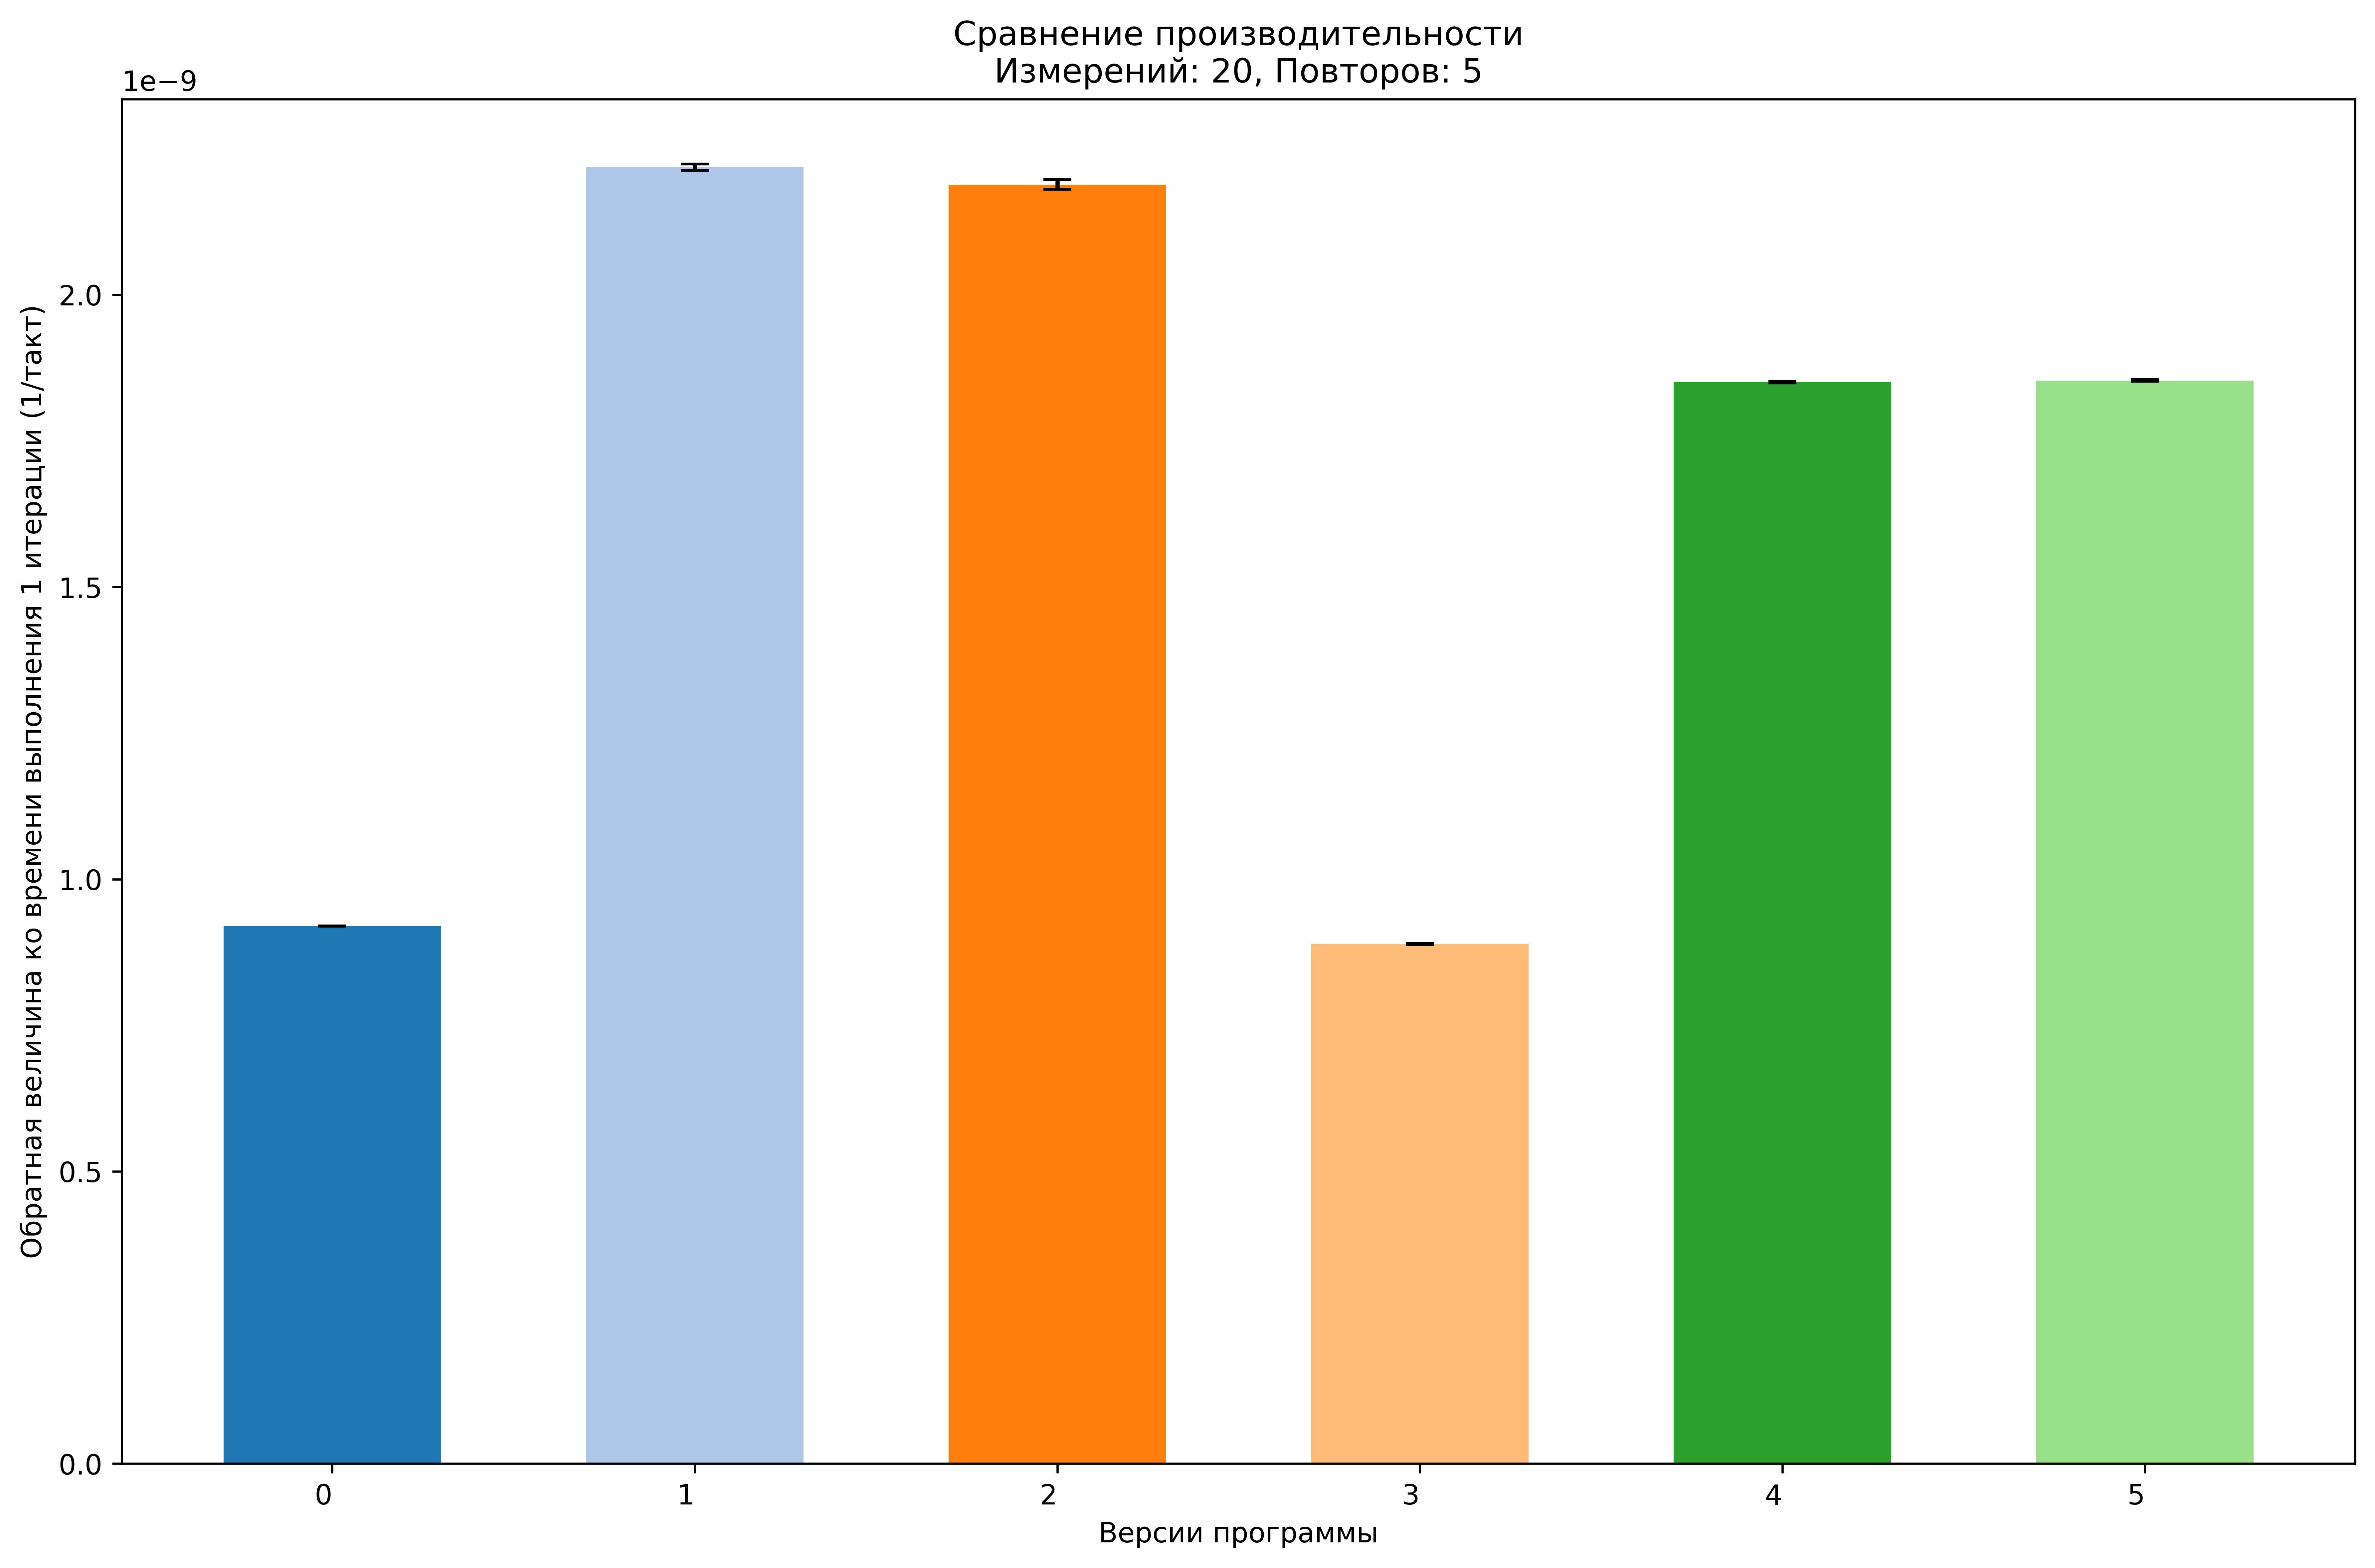
\includegraphics[width=0.8\textwidth]{histogram0.png}
    \caption{Гистограмма увеличения производительности наивными оптимизациями}
    \label{fig:histogram0}
\end{figure}

Над каждым столбиком гистограммы написано среднее время расчёта 1 кадра выраженное в тактах со среднеквадратичной погрешностью, а также прирост производительности относительно худшего результата. Как вы можете видеть, в лучшей конфигурации применялся уровень оптимизации -O2 и использовался компилятор gcc. Далее прирост производительности будем смотреть относительно этой версии.

\paragraph{Не наивные оптимизации.} Теперь посмотрим ускорение оставшихся версий программы.

\begin{figure}[ht!]
    \centering
    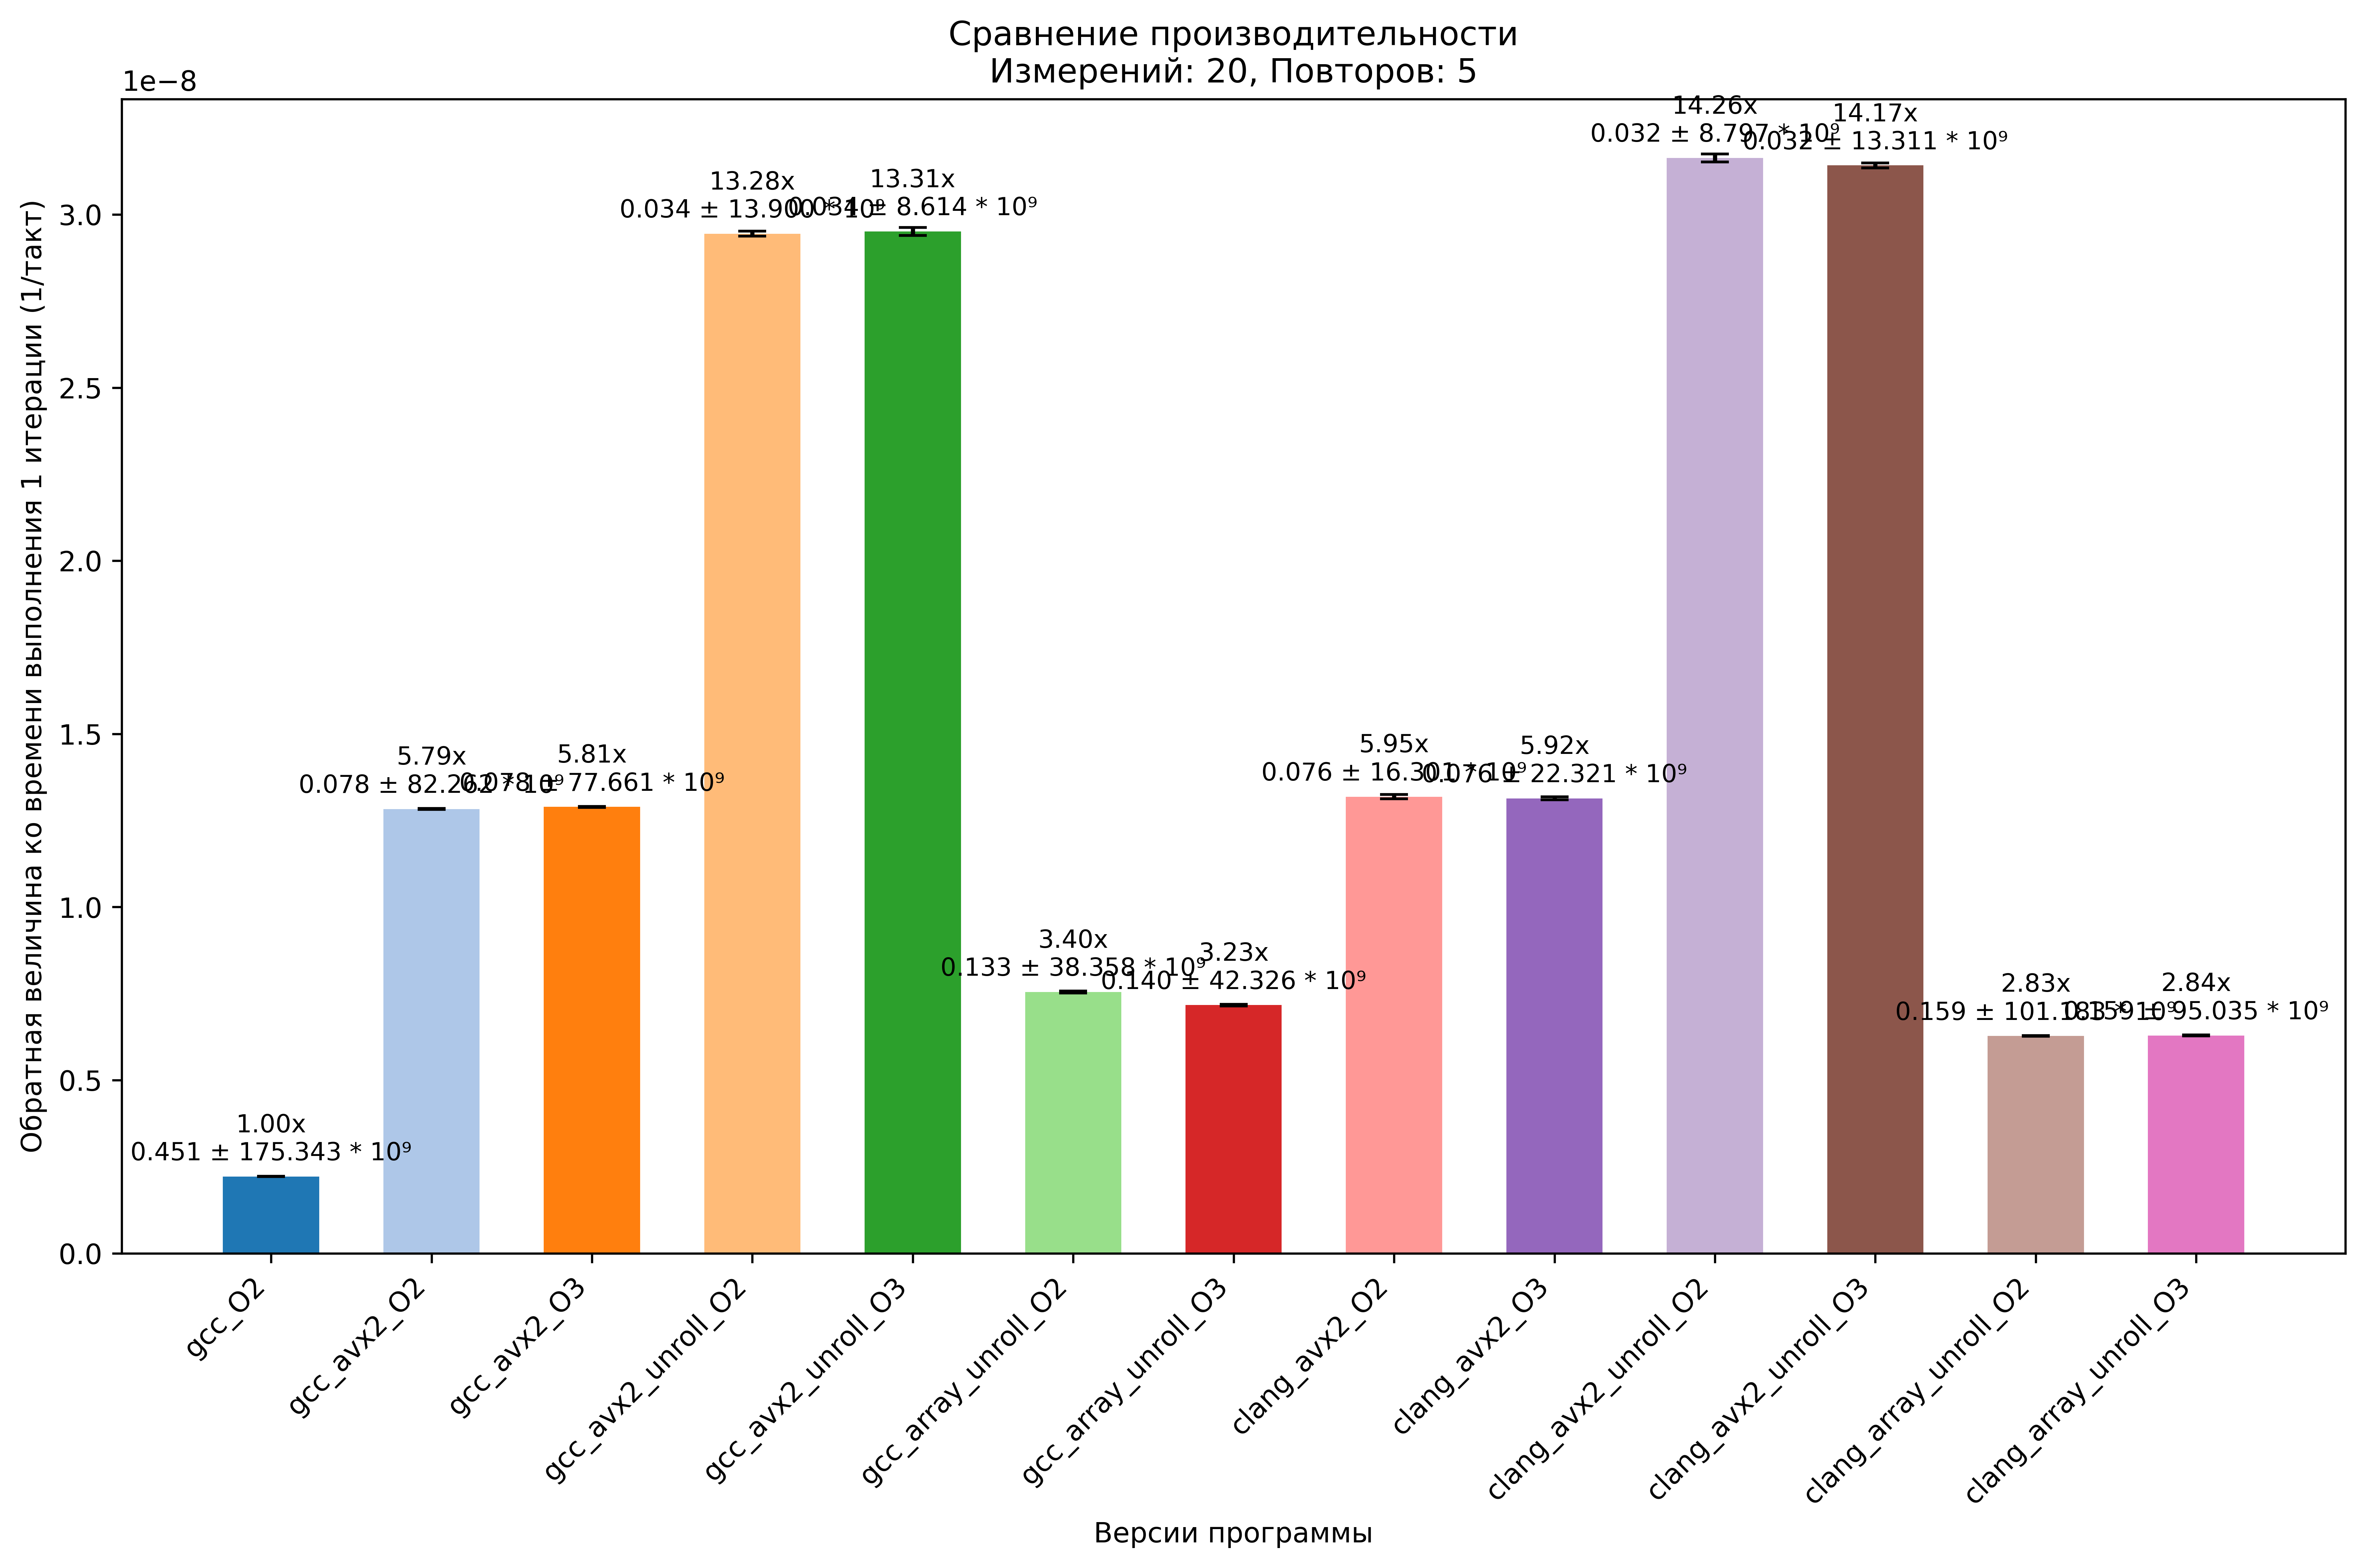
\includegraphics[width=0.7\textwidth]{histogram1.png}
    \caption{Гистограмма увеличения производительности не наивными оптимизациями}
    \label{fig:histogram1}
\end{figure}

Как вы можете видеть самой лучшей версией по производительности является та, в которой использовались векторные инструкции, реализованные через интринсики, с флагов оптимизации -O2 развёртыванием цикла на 4 и компилятором clang. Версии с флагом оптимизации -O3 могут показывать себя немного хуже, так как применяют агрессивные методы, которые могут ухудшить производительность.

Версия на массивах в данной работе показала плохую эффективность, по сравнению с непереносимыми аналогами. Это может быть связано с недостаточно очевидным для компилятора заменами интринсиков на массивы.

Ожидаемый прирост лучшей версии (в $8*4=32$ раза) в более чем 2 раза  больше того, что в итоге получился. Это можно объяснить тем, что наивный оптимизации обычной версии улучшали код именно в тех местах, которые мы заменили на векторные инструкции, при этом аналогичные оптимизации к векторам применить не удалось. При этом, если рассматривать прирост лучшей версии относительно той, в которой не было применено никаких оптимизаций, то прирост получается в $2.49*14.26\approx35.5$ раз, что коррелирует с предполагаемой эффективностью.

\section{Вывод}

В ходе выполнения данной работы была проведена комплексная оценка эффективности различных оптимизаций при вычислении множества Мандельброта. Основные этапы:

\subsection{Теоретический анализ}
\begin{itemize}
    \item Рассмотрены базовые модели выполнения инструкций (SEQ и PIPE), а также современные суперскалярные и конвейерные архитектуры
    \item Изучены методы оптимизации, включая вынос кода, уменьшение рисков по данным, развёртывание циклов, использование аккумуляторов и SIMD-инструкций
    \item Описаны способы измерения производительности, включая фиксацию тактовой частоты процессора и использование инструкции \texttt{rdtsc}
\end{itemize}

\subsection{Практическая реализация}
\begin{itemize}
    \item Разработана программа для визуализации множества Мандельброта с возможностью настройки параметров и отключения графики
    \item Последовательно применены различные оптимизации:
    \begin{itemize}
        \item Наивные (флаги компилятора \texttt{-O2}, \texttt{-O3}, PGO)
        \item Векторные инструкции (AVX2 через интринсики)
        \item Развёртывание циклов
        \item Кроссплатформенная реализация через массивы
    \end{itemize}
    \item Проведены тесты на стационарность процесса для обеспечения достоверности измерений
\end{itemize}

\subsection{Оценка производительности}
\begin{itemize}
    \item Наилучший результат показала версия с интринсиками, развёртыванием цикла на 4 порядка и компиляцией через \texttt{clang} с флагом оптимизации \texttt{-O2}
    \item Максимальный прирост производительности относительно базовой версии составил \textbf{$\sim$35.5 раз}, что близко к теоретически ожидаемому ускорению (32x)
    \item Оптимизации компилятора (\texttt{-O3}) в некоторых случаях ухудшали производительность из-за агрессивных преобразований
\end{itemize}

\subsection{Итоги}
\begin{itemize}
    \item SIMD-оптимизации обеспечили наибольший прирост производительности
    \item Развёртывание циклов и аккумуляторы дополнительно ускорили вычисления
    \item Кроссплатформенный подход на массивах показал более худшие результаты, но может быть полезен для переносимости
\end{itemize}

\textbf{Заключение:} Применение низкоуровневых оптимизаций (SIMD, развёртывание циклов) в сочетании с правильными флагами компиляции позволяет значительно ускорить вычисления. Однако эффективность зависит от архитектуры процессора и качества оптимизации компилятора. Для достижения максимальной производительности рекомендуется использовать аппаратно-зависимые инструкции (интринсики).

\section{Полезные ссылки}

\begin{enumerate}
    \item \href{https://github.com/kzueirf12345/mandelbrat2}{Сюда звёздочки ставить}
    \item \href{https://vk.com/wall-51126445_124413}{Компьютерные системы. Архитектура и программирование [2022] Брайант Р. Э., О'Халларон Д. Р.}
    \item \href{https://www.researchgate.net/figure/Data-Forwarding-1-With-a-forwarding-unit-these-stall-cycles-can-be-alleviated-See_fig2_308963446}{(Визуализация продвижения)}
    \item \href{https://www.laruence.com/sse/#techs=MMX,SSE,SSE2,SSE3,SSSE3,SSE4_1,SSE4_2,AVX,AVX2&expand=4974,4923,3865,3869,3870,736&text=mul}{Зеркало сайта с интрисинками на intel}
\end{enumerate}


\end{document}